\begin{recipe}
[% 
    preparationtime = {\unit[1.5]{h}},
    portion = {\portion{4}},
    bakingtime={\unit[0.5]{min}}
]
{Polish croquette with spinach and feta cheese}

    \ingredients[20]{%
       2 c. & Flour \\
       4 & Eggs \\
       2 c. & Milk \\
       1.5 c. & Water \\
       pinch & Salt \\
       2 tbs. & Oil \\
       & \\
       800 g & Spinach \\
       5 & Garlic cloves \\
       200 g & Feta cheese \\
       & Nutmeg \\
       & \\
       & Breadcrumbs \\
       & Beaten egg
    }

    \preparation{%
        \step Mix all ingredients for crepes batter. Fry crepes on a greased frying pan.
       
        \step Fry spinach, nutmeg and garlic till most of the water from spinach evaporates. Then add crushed feta cheese and mix well.
       
        \step Croquette folding - see picture.
        
        \begin{figure}[!h]
        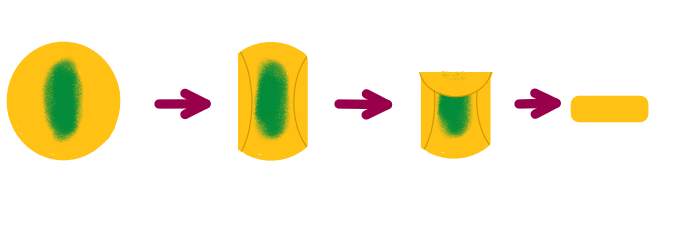
\includegraphics[width=.6\linewidth]{krokiety}
        \end{figure}
        
        \step Folded croquettes dip in beaten egg (with salt and pepper) and then cover with breadcrumbs. Fry till brown (you'll need relatively lots of oil).
    }

%  \graph
% {% pictures
% 	big=pic/krokiety  % big picture
% }

 \suggestion{%
	Now try different fillings. Maybe mushroom, pepper and cheddar?  
}

\end{recipe}